\documentclass{paper}

\usepackage{amsmath,amssymb,amsfonts, listings, fancyhdr, stmaryrd, array, tikz}
\usepackage[many]{tcolorbox}
\usepackage[a4paper, total={170mm,257mm}, left=20mm, top=20mm]{geometry}
\newtheorem{prop}{Proposition}
\newtheorem{defi}{Definition}
\newtheorem{preuve}{Preuve}

\newcolumntype{C}{>$c<$}
\tcolorboxenvironment{prop}{enhanced, borderline={0.8pt}{0pt}{blue}, borderline={0.4pt}{2pt}{cyan}, boxrule=0.4pt, colback=white, coltitle=black, sharp corners}
\tcolorboxenvironment{defi}{ enhanced, borderline={0.8pt}{0pt}{red}, borderline={0.4pt}{2pt}{orange}, boxrule=0.4pt, colback=white, coltitle=black, sharp corners}
\tcolorboxenvironment{preuve}{ enhanced, borderline={0.8pt}{0pt}{green}, borderline={0.4pt}{2pt}{lime}, boxrule=0.4pt, colback=white, coltitle=black, sharp corners}

\pagestyle{fancy}
\fancyhead[C]{TIPE 25/26 - Dorian GIL}

\begin{document}
\setlength{\headheight}{13.07225pt}
\addtolength{\topmargin}{-1.07225pt}

\section*{Méthode des tableaux : Optimisation}
memoisation, SQL, dictionnaire, serialisation

\tableofcontents





\section{Logique Propositionelle}

\subsection{Definition}



\begin{defi}
La \textit{logique propositionelle} est un type de logique où les formules sont obtenus par des variables propositionelles reliées par des connecteurs.
\end{defi}
\begin{defi}[Modèle]
    Un \textit{modèle} d'une formule $\phi$ est une valuation qui rend vraie cette formule. On note l'ensemble des modèles de $\phi$ par:
    $$Mod(\phi) := \{v\in Val | v \vDash \phi\}$$
    $Val$ étant l'ensemble des valuations de $\phi$ et $v \vDash \phi$ signfiant que la valuation $v$ satisfait $\phi$
\end{defi}
\begin{defi}[Conséquence Logique]
    Une formule $\phi$ est \textit{conséquence logique} d'une formule, notée $\psi$ si $Mod(\psi) \subseteq Mod(\phi)$. On note cela $\psi \vDash \phi$
\end{defi}

\begin{defi}[Arbre de déduction]
    Arbre dont les sommets sont composés de formule, qui sont soit une hypothèse à la racine de l'arbre, soit une formule obtenue par l'application d'une règle sur une formule présente dans la même branche plus proche de la racine.
\end{defi}

\begin{defi}[Branche fermée]
    Une branche est fermée si elle contient $\phi$ et $\lnot\phi$
\end{defi}

\begin{defi}[Arbre fermé]
    Un arbre de déduction est fermé si toutes les branches le sont.
\end{defi}



\subsection{Principe}
On note $n\in\mathbb{N}^*$, le procédé de la méthode des tableaux consiste donc à séparer les formules logiques complexes en plus petite formule jusqu'à que des pairs complementaires de litteraux ($a$ et $\lnot a$) soit extrait ou qu'on ne peut plus simplifier la formule.
On en déduit ainsi si une formule $\phi$ est insatisfaisable ou pas en adoptant des règles qu'on applique sur un arbre de déduction.
\begin{itemize}
    \item On place $\lnot\phi$ dans la racine de l'arbre.
    \item On applique les règles $(R_x)$ suivantes à chaque branche non fermé de l'arbre
    \item Si l'arbre est in fine fermé, alors $\phi$ est vrai
\end{itemize}

Les règles $(R_x)$ dites Smullyan-style sont:

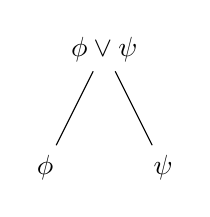
\begin{tikzpicture}
\node {$\phi\lor\psi$}
    child {node {$\phi$}}
    child {node {$\psi$}};
\end{tikzpicture}
$(R_\lor)$
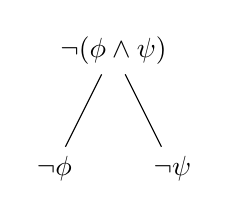
\begin{tikzpicture}
\node {$\lnot(\phi\land\psi)$}
    child {node {$\lnot\phi$}}
    child {node {$\lnot\psi$}};
\end{tikzpicture}
$(R_{\lnot\land})$
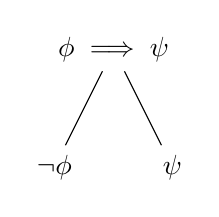
\begin{tikzpicture}
\node {$\phi\implies\psi$}
    child {node {$\lnot\phi$}}
    child {node {$\psi$}};
\end{tikzpicture}
$(R_{\implies})$
\begin{tikzpicture}
\node {$\lnot\lnot\phi$}
    child {node {$\phi$}};
\end{tikzpicture}
$(R_{\lnot\lnot})$
\begin{tikzpicture}[level distance=8mm]
\node {$\phi\land\psi$}
    child {node {$\phi$} edge from parent }{
    child {node {$\psi$} edge from parent[draw=none]}};
\end{tikzpicture}
$(R_{\land})$

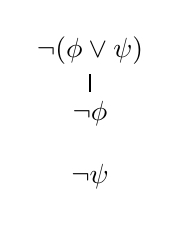
\begin{tikzpicture}[level distance=8mm]
\node {$\lnot(\phi\lor\psi)$}
    child {node {$\lnot\phi$} edge from parent }{
    child {node {$\lnot\psi$} edge from parent[draw=none]}};
\end{tikzpicture}
$(R_{\lnot\lor})$
\begin{tikzpicture}[level distance=8mm]
\node {$\lnot(\phi\implies\psi)$}
    child {node {$\phi$} edge from parent }{
    child {node {$\lnot\psi$} edge from parent[draw=none]}};
\end{tikzpicture}
$(R_{\lnot\implies})$
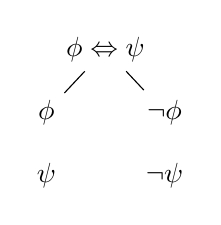
\begin{tikzpicture}[level distance=8mm]
\node {$\phi\Leftrightarrow\psi$}
    child {node {$\phi$} 
        child {node {$\psi$} edge from parent[draw=none]}}
    child {node {$\lnot\phi$}
        child {node {$\lnot\psi$} edge from parent[draw=none]}};
\end{tikzpicture}
$(R_{\Leftrightarrow})$
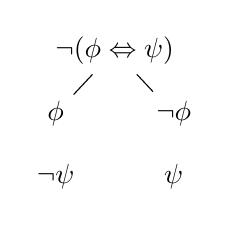
\begin{tikzpicture}[level distance=8mm]
\node {$\lnot(\phi\Leftrightarrow\psi)$}
    child {node {$\phi$} 
        child {node {$\lnot\psi$} edge from parent[draw=none]}}
    child {node {$\lnot\phi$}
        child {node {$\psi$} edge from parent[draw=none]}};
\end{tikzpicture}
$(R_{\lnot\Leftrightarrow})$

Dans les cas où on trouve dans une même branche $a$ et $\lnot a$, on ferme la branche, si l'arbre devient fermé, alors $\lnot\phi$ est forcement faux, donc $\phi$ est forcement vrai.

\begin{prop}
    Soit $\Psi$ un ensemble d'hypothèse et $\phi$ une formule, on note $\Psi\vdash\phi$ l'existence d'un arbre fermé pour $\Psi\cup\{\lnot\phi\}$.
    $$\Psi\vdash\phi \Leftrightarrow \Psi\vDash\phi$$
    Autrement dit, appliqué la méthode des tableaux à la négation de la formule et ses hypothèses est équivalent à prouver cette formule (\textit{Prouver dans le sens que c'est une tautologie en suppossant $\Psi$})
\end{prop}

\begin{preuve}
    La preuve de cette proposition permet de prouver la correction de l'implémentation de base.
    Elle est trouvable en ligne
\end{preuve}
Cette proposition assure un moyen de prouver une formule.

\begin{prop}
    Soit $\Psi$ un ensemble d'hypothèse et $\phi$ une formule, on note $\Psi\vdash\phi$ la non existence d'un arbre fermé pour $\Psi$.
    $$\Psi\vdash\phi \Leftrightarrow \Psi\vDash\phi$$
    Autrement dit, appliqué la méthode des tableaux est équivalent à prouver la satisfaisabilité de cette formule
\end{prop}

\begin{preuve}
    En ligne
\end{preuve}
Cette proposition assure un moyen de prouver la satisfaisabilité d'une formule



\subsection{Formules de forme alternée}

\begin{defi}
Soit $n\in\mathbb{N}^*$ et $(\alpha_k)_{k\in[|1, n|]}$ des litteraux, une formule $\phi$ est de forme alternée ssi
$$\phi := \alpha_1 \land (\alpha_2 \lor (\alpha_3 \land (\dots (\alpha_n))))$$
\end{defi}
On gardera les parenthèses dans la suite pour garder le coté intuitif de cet ecriture et surtout ne pas laisser l'ambiguité sur la prioritée entre les opérateurs logiques


On remarque une CNS pour que ce type de formule soit vrai:
\begin{prop}[CNS - A reformuler]
    $\phi$ de forme alternée est vrai ssi:
    $$(\exists k\in\mathbb{N}^*, \alpha_{2k-2} \text{ OU n impair}\implies\alpha_n \text{ avec } k=\frac{n-1}{2})\text{ ET } \forall i\in[|1, k|], \alpha_{2i-1}$$
\end{prop}

\begin{preuve}
    $(\impliedby)$ Immédiat
    
    $(\implies)$ Supposons $\phi$ de forme alternée vrai:
    $\alpha_1$ est forcement vrai, deux possibilités :
    soit $\alpha_2$ est vrai, soit $\alpha_3\land(\dots)$ est vrai. Dans le deuxième cas, on repète le raisonnement sur $\alpha_3\land(\dots)$ qui est bien de forme alternée.
    
    Deux cas de figure:
    \begin{itemize}
        \item On arrête donc le processus dès que un litteral indéxée par un nombre pair est vrai.
        Dans ce cas là, tout les indéxées impair précedents sont aussi vrai.
        \item Si aucun litteral pair est vrai, alors $n$ est impair sans quoi $\phi$ n'est pas vrai car $\alpha_n$ doit être vrai. 
        On en déduit que tout les litteraux impairs sont vraies, donc la formule est vrai.
    \end{itemize}    
\end{preuve}

Mais ceci n'est pas important, cela aide juste à se donner une idée de la structure de la formule, pour trouver des CNS plus intéressantes.


\subsection{Satisfaisabilité}
On rappelle que pour prouver la satisfaisabilité d'une formule, on montre qu'il n'existe pas d'arbre fermé.
Revenons à la méthode des tableaux, en appliquant les règles à la famille de formule de forme alternée,
on observe un patterne sur l'arbre résultant $\forall k\in\mathbb{N}^*$:

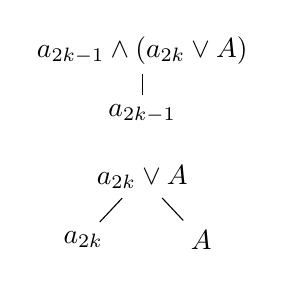
\begin{tikzpicture}[level distance=8mm]
    \node {$a_{2k-1}\land(a_{2k}\lor A)$}
        child {node {$a_{2k-1}$} edge from parent }{
        child {node {$a_{2k}\lor A$}
        child {node {$a_{2k}$}}
        child {node {$A$}}; edge from parent[draw=none]}};
\end{tikzpicture}

où $A$ est la suite de la forme alternée, qui est aussi de forme alterné ou un littéral.

\begin{prop}
   Chaque arbre induit par la méthode des tableaux est un arbrre binaire, tel qu'on nomme dans les nodes les hypothèses à l'étape associé de l'algorithme
\end{prop}

\begin{preuve}
    Soit $A_1$ et $A_2$ deux arbres binaires représentant l'arbre induit par la méthode des tableaux $T_1$ et $T_2$ respectivement, etiquetés par des litteraux, on suppose qu'ils sont égaux. On peut les reconstruire par une succession d'opération sur une formule par la méthode des tableaux.
    Etant donné que $A_1=A_2$, on applique les mêmes opérations, sans quoi on aura pas les mêmes arbres binaires, donc on a la même formule et les mêmes hypothèses, donc $T_1=T_2$
\end{preuve}

L'arbre induit ; pour $n=5$ ; et pour $n=4$

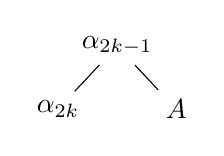
\begin{tikzpicture}[level distance=8mm]
    \node {$\alpha_{2k-1}$}
        child {node {$\alpha_{2k}$}}
        child {node {$A$}};
\end{tikzpicture}
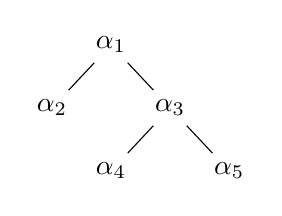
\begin{tikzpicture}[level distance=8mm]
    \node {$\alpha_1$}
        child {node {$\alpha_2$}}
        child {node {$\alpha_3$}
        child {node {$\alpha_4$}}
        child {node {$\alpha_5$}}};
\end{tikzpicture}
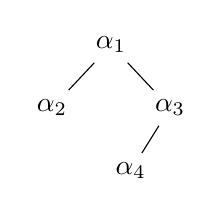
\begin{tikzpicture}[level distance=8mm]
    \node {$\alpha_1$}
        child {node {$\alpha_2$}}
        child {node {$\alpha_3$}
            child [xshift=-5mm]{node {$\alpha_4$}}};
\end{tikzpicture}

Faisons des raisonnements pour des formules de taille $n\in [|1, 3|]$:
\begin{enumerate}
    \item Toujours satisfaisable
    \item Satisfaisable ssi $\alpha_2 \neq \lnot\alpha_1$
    \item Satisfaisable ssi $\lnot(\alpha_1 = \lnot\alpha_2 = \lnot\alpha_3)$
\end{enumerate}
C'est à partir du cas $n=4$ que la satisfaisabilité devient difficile à retablir. On peut l'établir par 2-SAT, et trouver qu'il y a 
4096 formules possibles avec 168 d'entres elles qui sont insatisfaisable, on sent que trouver une CNS peut être compliqué, surtout quand
on va prendre des $n$ plus hauts











\subsection{Preuve sous hypothèse}

\begin{prop}
    Avec les mêmes définitions, soit $\phi = \alpha_1 \land (\alpha_2 \lor (\alpha_3 \land (\dots (\alpha_n))))$ une formule de formule alternée:
    $$\lnot\phi = \lnot\alpha_1 \lor (\lnot\alpha_2 \land (\lnot\alpha_3 \lor (\dots (\lnot\alpha_n))))$$
\end{prop}
Cette forme est cohérente avec les propriétés de $\lnot$.

\begin{preuve}
    On prouve par recurrence forte sur $n\in\mathbb{N}^*$

    $\mathcal{P}(n): \lnot\phi = \lnot\alpha_1 \lor (\lnot\alpha_2 \land (\lnot\alpha_3 \lor (\dots (\lnot\alpha_n))))$

    $\mathcal{P}(1): \lnot\phi = \lnot\alpha_1$ vrai

    $\forall k\in\mathbb{N}^*$, supposons $\mathcal{P}(k)$:

    $\lnot\phi = \lnot (\alpha_1 \land (\alpha_2 \lor (\alpha_3 \land (\dots (\alpha_{n+1})))))$

    $= \lnot\alpha_1 \lor (\lnot\alpha_2 \land \lnot(\alpha_3 \land (\dots (\alpha_{n+1}))))$

    On trouve le résultat en appliquant l'hypothèse de recurrence sur $\alpha_3 \land (\dots (\alpha_{n+1}))$ qui est de forme alternée.

    $\forall n\in\mathbb{N}^*, \mathcal{P}(n)$
\end{preuve}

De là, on peut enfin en déduire la forme de l'arbre induit par la méthode des tableaux sur la négation d'une formule de forme alternée sans hypothèse

\begin{tikzpicture}
\node {$\lnot\alpha_1\lor(\lnot\alpha_2\land \lnot A)$}
    child {node {$\lnot\alpha_1$}}
    child {node {$\lnot\alpha_2\land\lnot A$}
        child {node {$\lnot\alpha_2$}}{
        child {node {$\lnot A$} edge from parent[draw=none]}
        }
    };
\end{tikzpicture}

\begin{prop}
    $\lnot\phi$ de forme alternée est vrai ssi:
    $$(\forall k\in\mathbb{N}^*, \lnot\alpha_{2k-2} \text{ ET n impair ET } \lnot\alpha_n \text{ avec } k=\frac{n-1}{2}) \text{ OU } \exists i\in [|1,k], \lnot\alpha_{2i-1}$$
\end{prop}

\begin{preuve}
    On utilise la négation de la proposition 3 ainsi que $\phi \rightarrow F \Leftrightarrow \lnot\phi \rightarrow T$  
\end{preuve}



























\section{Logique du 1er ordre}
La logique propositionelle étant mathématiquement limité, on se propose l'utilisation de la logique du 1er ordre.
Cela nous permettra ainsi d'étudier Zenon, un prouveur d'automatique de theorème.
\begin{defi}
    La \textit{logique du 1er ordre} est un type de logique qui en plus des élements de la logique propositionelle permet l'utilisation de
    quantificateurs et de \textit{termes}.
\end{defi}

\begin{defi}
    Soit un ensemble infini de variables $X = \{x,y,x_1,x_2,\dots \}$ et un ensemble $\mathcal{F}=\{c,f,g,\dots \}$ de symboles de fonction (autrement appelé signature).
    On rappelle que l'arité d'un symbole est son nombre d'argument.
    Les termes sont définis par induction:
    \begin{itemize}
        \item $\forall x\in X, x$ est un terme
        \item Tout symbole d'arité $0$ (les constantes) est un terme
        \item $f(t_1,\dots,t_n)$ est un terme ssi $f$ est un symbole d'arité $n$ et $t_1,\dots,t_n$ sont des termes
    \end{itemize} 
    On note $\mathcal{T}(\mathcal{F}, X)$ l'ensemble des termes sur $\mathcal{F}$ et $X$.
\end{defi}



\end{document}